\section{Development and Runtime Environment}

\subsection{Software development environment}

The avl compiler was developed under Unix-based environments. Our goal is to make a compiler highly
portable on all Unix-based environments, including Linux and Mac OS. In addition, we made full use
of Git and GitHub for reliable version control.

Flex is used to create the scanner, which reads the source file and generates a stream of tokens.
The parser is created by Bison. Combined with the code generator, we generate c++ target code. The
output c++ file is formatted by a tool called astyle and finally compiled by g++.

\subsection{Makefile}

We use GNU Autotools (autoconf/automake/libtool...) to generate \verb"Makefile"s automatically.
Autotools help us create \verb"Makefile"s that are fully GNU standards-compliant and extremely easy
to maintain.

For developers, we only need to create the following files to specify how the \verb"Makefile"s will
be generated:

\begin{itemize}
  \item \verb"configure.ac" in the top level directory
  \item \verb"Makefile.am"s in directories where \verb"Makefile"s are needed.
\end{itemize}

In order to create Makefiles, all the develop needs to do is to run the following commands:

\begin{verbatim}
    autoreconf --install
    ./configure
\end{verbatim}

Another significant feature provided by Autotools is that running test cases can be as easy as
typing a single command:

\begin{verbatim}
    make check
\end{verbatim}

As we can see from Fig.~\ref{fig:automake}, the report tells us which of the test cases passed and which of the test cases
failed. Each test script would write the output into a log file, so we are able to identify the
error message from the corresponding log file.

\begin{figure}[htp]
  \centering
  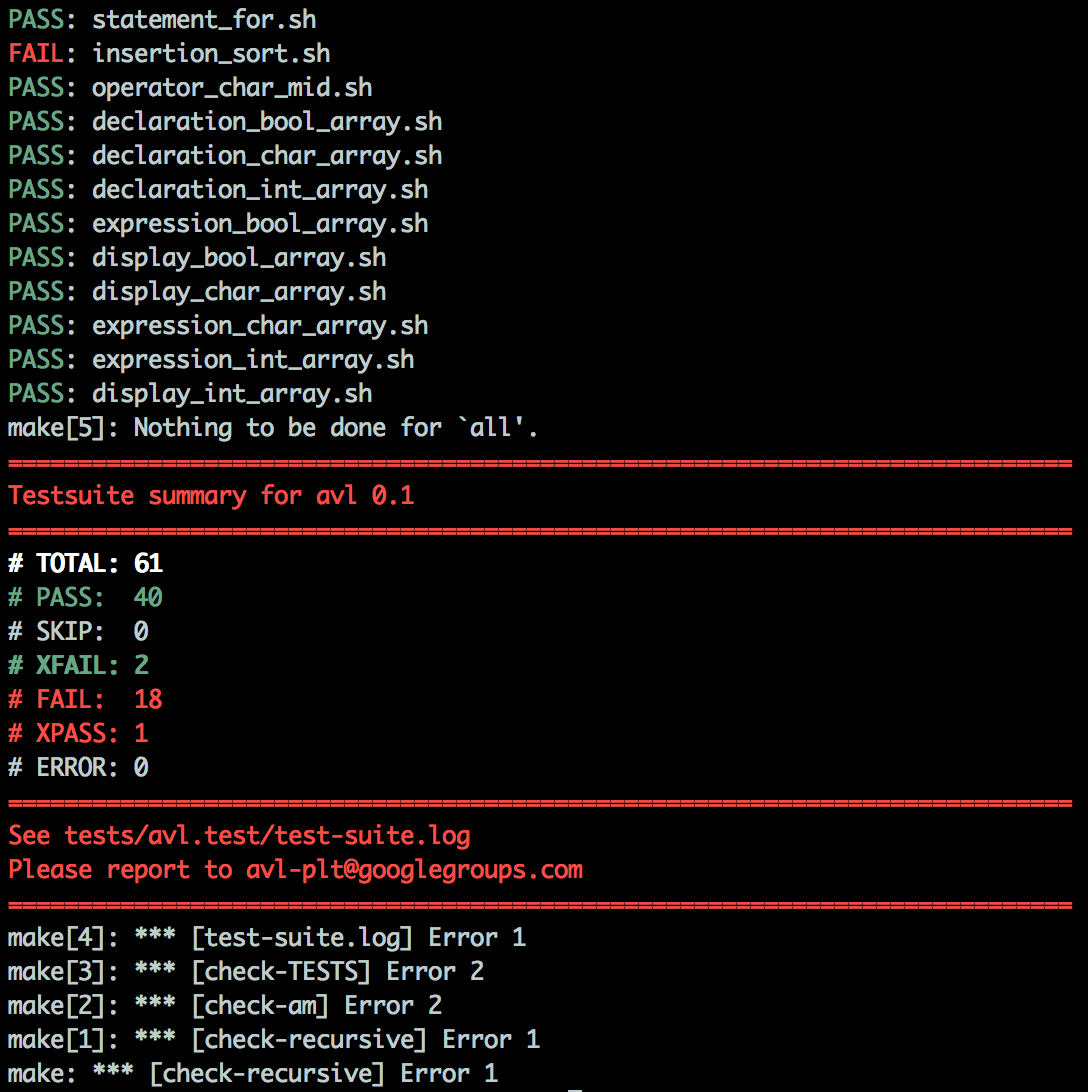
\includegraphics[height=12cm]{automake.png}
  \caption{Automated testing}
  \label{fig:automake}
\end{figure}

All the \verb"Makefile"s are listed below.

\paragraph{configure.ac}

\begin{verbatim}
AC_INIT([avl], [0.1], [avl-plt@googlegroups.com], [],
[https://github.com/wqfish/avl])

AM_INIT_AUTOMAKE([-Wall -Werror foreign])

AC_PROG_CC
AC_PROG_CXX
AC_PROG_LEX
AC_PROG_YACC

AC_CONFIG_MACRO_DIR([m4])
AM_PROG_AR
AC_PROG_LIBTOOL

AC_CONFIG_HEADERS([config.h])
AC_CONFIG_FILES([
         Makefile
         src/Makefile
         lib/Makefile
         sample_code/Makefile
         tests/Makefile
         tests/libavl.test/Makefile
         tests/avl.test/Makefile
         tests/error.test/Makefile
])

AC_OUTPUT
\end{verbatim}

\paragraph{Makefile.am}

\begin{verbatim}
ACLOCAL_AMFLAGS = -I m4
SUBDIRS = src lib sample_code tests
\end{verbatim}

\paragraph{src/Makefile.am}

\begin{verbatim}
BUILT_SOURCES = parser.h
AM_YFLAGS = -d
bin_PROGRAMS = avl
avl_SOURCES = scanner.l parser.y avl.c syntax_tree.c code_generator.c sym_list.c sym_table.c
st_list.c
AM_CFLAGS = -Werror
\end{verbatim}

\paragraph{lib/Makefile.am}

\begin{verbatim}
lib_LTLIBRARIES = libavl.la
libavl_la_SOURCES = AvlVisualizer.cpp
include_HEADERS = AvlVisualizer.h AvlTypes.h AvlUtils.h
AM_CPPFLAGS = -Wall -Wextra -Werror -std=c++11 -I/opt/local/include
\end{verbatim}

\paragraph{sample\_code/Makefile.am}

\begin{verbatim}
noinst_PROGRAMS = sorting merge_sorted_array
sorting_SOURCES = sorting.cpp
merge_sorted_array_SOURCES = merge_sorted_array.cpp

AM_CPPFLAGS = -Wall -Werror -std=c++11 -I$(top_builddir)/lib -I/opt/local/include
AM_LDFLAGS = -L$(top_builddir)/lib -L/opt/local/lib -lavl -lGL -lglut
\end{verbatim}

\paragraph{tests/Makefile.am}

\begin{verbatim}
SUBDIRS = libavl.test avl.test error.test

tests/libavl.test/Makefile.am
check_PROGRAMS = \
                 avlint_assign1 \
                 avlint_add1 \
                 avlint_add2 \
                 avlint_add3 \
                 avlint_sub1

avlint_assign1_SOURCES = avlint_assign1.cpp
avlint_add1_SOURCES = avlint_add1.cpp
avlint_add2_SOURCES = avlint_add2.cpp
avlint_add3_SOURCES = avlint_add3.cpp
avlint_sub1_SOURCES = avlint_sub1.cpp

AM_CPPFLAGS = -Wall -Werror -std=c++11 -I$(top_builddir)/lib -I/opt/local/include
AM_LDFLAGS = -L$(top_builddir)/lib -L/opt/local/lib -lavl -lglut -lGL

AM_TESTS_ENVIRONMENT = . $(srcdir)/init_test.sh;
AM_TESTS_FD_REDIRECT = 9>&2

TESTS = \
        avlint_assign1.sh \
        avlint_add1.sh \
        avlint_add2.sh \
        avlint_add3.sh \
        avlint_sub1.sh
\end{verbatim}

\paragraph{tests/avl.test/Makefile.am}

\begin{verbatim}
AM_TESTS_ENVIRONMENT = . $(srcdir)/init_test.sh;
AM_TESTS_FD_REDIRECT = 9>&2

TESTS = \
        cast.sh \
        constant.sh \
        declaration_bool.sh \
        declaration_bool_array.sh \
        other_test_cases omitted...
        maxSubarray.sh

XFAIL_TESTS = \
        cast.sh \
        statement_scope.sh \
        empty.sh
\end{verbatim}

\paragraph{tests/error.test/Makefile.am}

\begin{verbatim}
AM_TESTS_ENVIRONMENT = . $(srcdir)/init_test.sh;
AM_TESTS_FD_REDIRECT = 9>&2

TESTS = \
        func_malformat.sh \
        func_malparam.sh \
        func_malscope.sh \
        other_test_cases omitted...
        array_malvalue.sh

XFAIL_TESTS = \
        func_malformat.sh \
        func_malparam.sh \
        other_test_cases omitted...
        array_malvalue.sh
\end{verbatim}

For users who want to use the compiler, in its simplest scenario, all the user has to do is to
unpack the package, then run the following commands:

\begin{verbatim}
    ./configure
    make
    sudo make install
\end{verbatim}

According to GNU standards, the avl compiler is installed to \verb"/usr/local/bin", header files to
\verb"/usr/local/include" and libraries to \verb"/usr/local/lib". Thus, after the installation the
user would be able to invoke avl from the command line.

\subsection{Runtime Environment}

As discussed above, the avl compiler works on all Unix-based systems, including Linux and Mac OS.
The latest version of the following tools are required:

\begin{itemize}
  \item gcc
  \item astyle
  \item OpenGL libraries: freeglut glew glm glfw
\end{itemize}

For Mac, an X window system is also required (\url{https://xquartz.macosforge.org/}).

The avl compiler can be invoked as follows:

\begin{verbatim}
    $ avl --help
    Usage: avl [-h|-o|-t] file
    Options:
      -h --help            Display this information
      -o --output=<file>   Compile and place the executable into <file>
      -t --translate       Translate the source files into c++
                              xxx.avl -> xxx.cpp
    Use at most one option at a time.

    For bug reporting instructions, please see:
    <https://github.com/wqfish/avl>.
\end{verbatim}
